% Created by tikzDevice version 0.12.6 on 2025-09-21 16:30:26
% !TEX encoding = UTF-8 Unicode
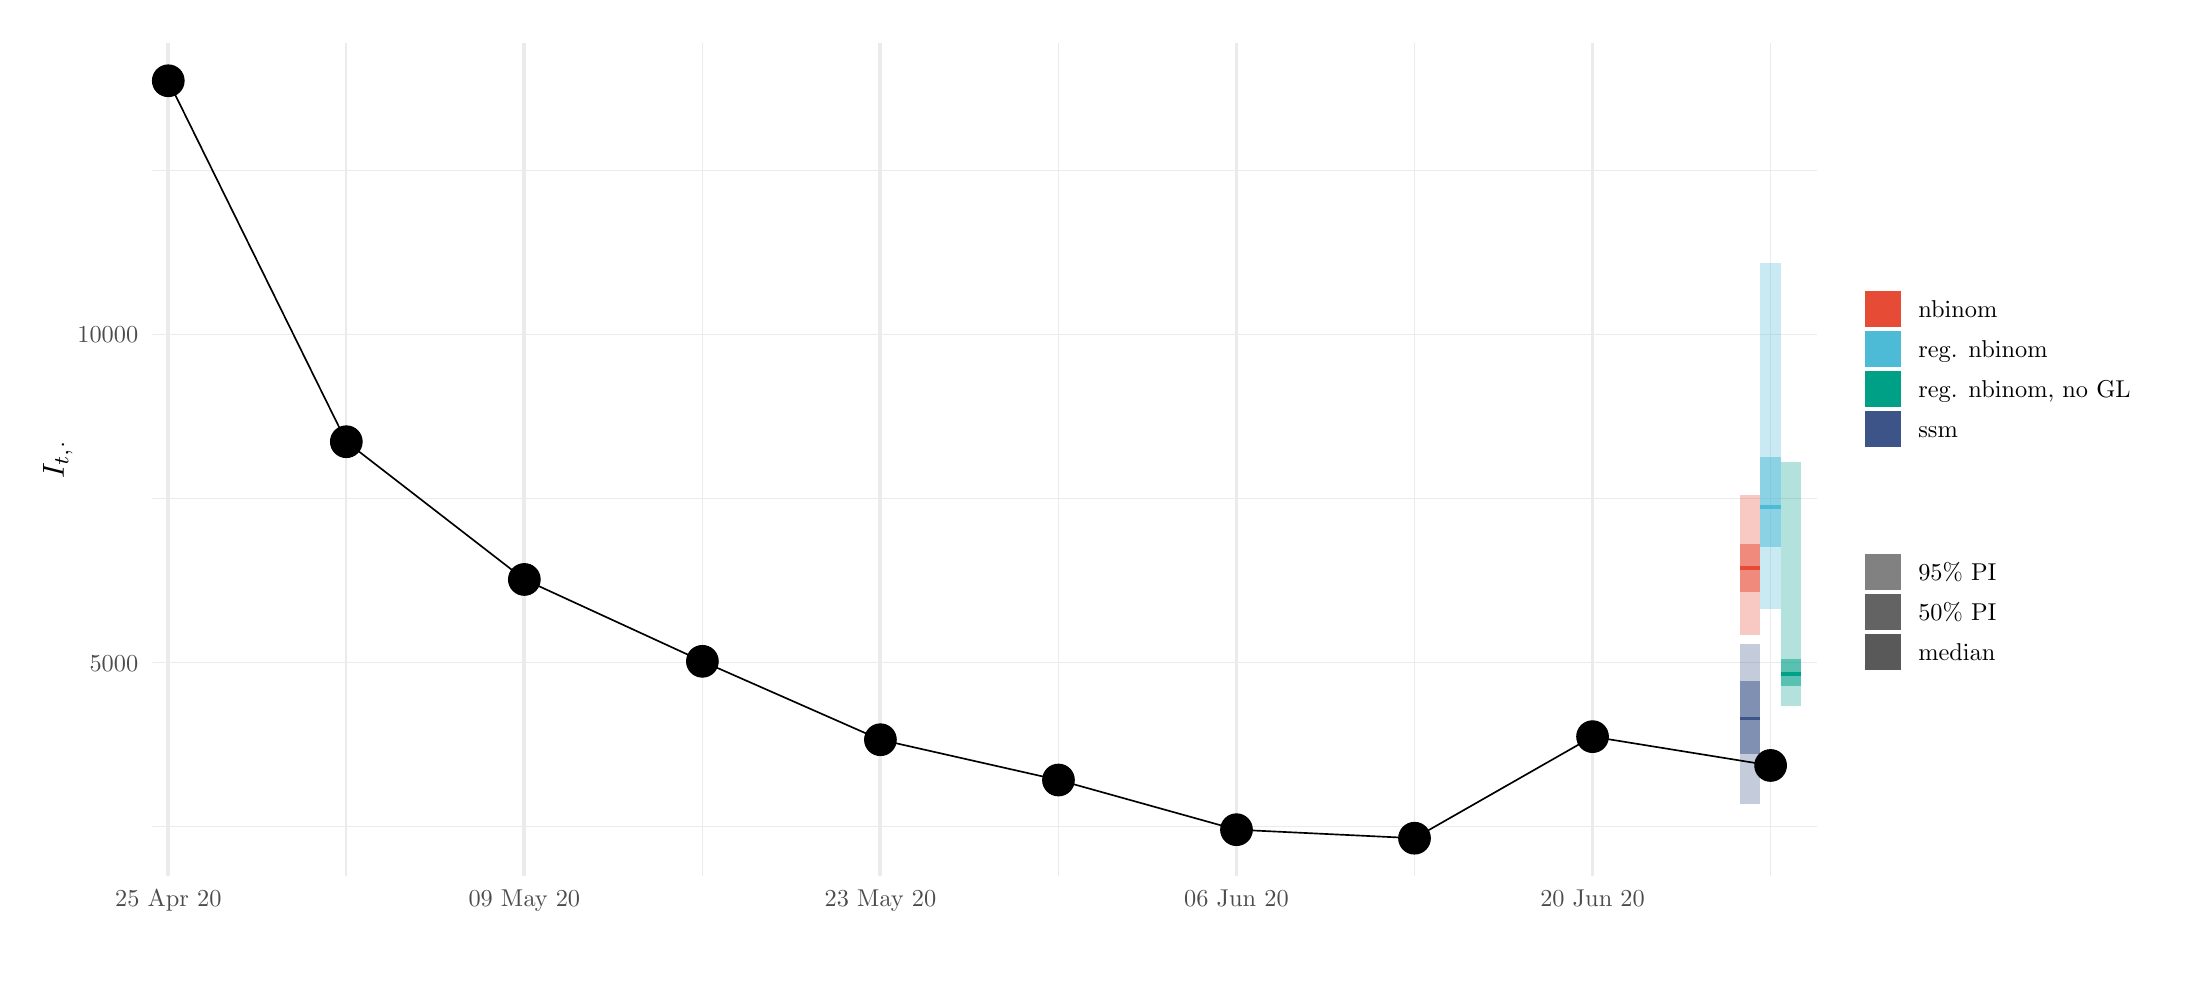
\begin{tikzpicture}[x=1pt,y=1pt]
\definecolor{fillColor}{RGB}{255,255,255}
\path[use as bounding box,fill=fillColor,fill opacity=0.00] (0,0) rectangle (770.88,337.26);
\begin{scope}
\path[clip] ( 44.91, 30.69) rectangle (646.73,331.76);
\definecolor{drawColor}{gray}{0.92}

\path[draw=drawColor,line width= 0.3pt,line join=round] ( 44.91, 48.54) --
	(646.73, 48.54);

\path[draw=drawColor,line width= 0.3pt,line join=round] ( 44.91,167.08) --
	(646.73,167.08);

\path[draw=drawColor,line width= 0.3pt,line join=round] ( 44.91,285.62) --
	(646.73,285.62);

\path[draw=drawColor,line width= 0.6pt,line join=round] (115.14, 30.69) --
	(115.14,331.76);

\path[draw=drawColor,line width= 0.6pt,line join=round] (243.81, 30.69) --
	(243.81,331.76);

\path[draw=drawColor,line width= 0.6pt,line join=round] (372.47, 30.69) --
	(372.47,331.76);

\path[draw=drawColor,line width= 0.6pt,line join=round] (501.13, 30.69) --
	(501.13,331.76);

\path[draw=drawColor,line width= 0.6pt,line join=round] (629.80, 30.69) --
	(629.80,331.76);

\path[draw=drawColor,line width= 0.6pt,line join=round] ( 44.91,107.81) --
	(646.73,107.81);

\path[draw=drawColor,line width= 0.6pt,line join=round] ( 44.91,226.35) --
	(646.73,226.35);

\path[draw=drawColor,line width= 1.4pt,line join=round] ( 50.81, 30.69) --
	( 50.81,331.76);

\path[draw=drawColor,line width= 1.4pt,line join=round] (179.47, 30.69) --
	(179.47,331.76);

\path[draw=drawColor,line width= 1.4pt,line join=round] (308.14, 30.69) --
	(308.14,331.76);

\path[draw=drawColor,line width= 1.4pt,line join=round] (436.80, 30.69) --
	(436.80,331.76);

\path[draw=drawColor,line width= 1.4pt,line join=round] (565.46, 30.69) --
	(565.46,331.76);
\definecolor{fillColor}{RGB}{60,84,136}

\path[fill=fillColor,fill opacity=0.30] (618.77, 56.66) rectangle (626.12,114.40);
\definecolor{fillColor}{RGB}{60,84,136}

\path[fill=fillColor,fill opacity=0.50] (618.77, 74.77) rectangle (626.12,101.23);
\definecolor{fillColor}{RGB}{60,84,136}

\path[fill=fillColor] (618.77, 86.92) rectangle (626.12, 88.35);
\definecolor{fillColor}{RGB}{230,75,53}

\path[fill=fillColor,fill opacity=0.30] (618.77,117.91) rectangle (626.12,168.55);
\definecolor{fillColor}{RGB}{230,75,53}

\path[fill=fillColor,fill opacity=0.50] (618.77,133.32) rectangle (626.12,150.72);
\definecolor{fillColor}{RGB}{230,75,53}

\path[fill=fillColor] (618.77,141.15) rectangle (626.12,142.57);
\definecolor{fillColor}{RGB}{77,187,213}

\path[fill=fillColor,fill opacity=0.30] (626.12,127.30) rectangle (633.47,252.19);
\definecolor{fillColor}{RGB}{77,187,213}

\path[fill=fillColor,fill opacity=0.50] (626.12,149.44) rectangle (633.47,182.11);
\definecolor{fillColor}{RGB}{77,187,213}

\path[fill=fillColor] (626.12,163.41) rectangle (633.47,164.83);
\definecolor{fillColor}{RGB}{0,160,135}

\path[fill=fillColor,fill opacity=0.30] (633.47, 92.17) rectangle (640.83,180.41);
\definecolor{fillColor}{RGB}{0,160,135}

\path[fill=fillColor,fill opacity=0.50] (633.47, 99.21) rectangle (640.83,109.12);
\definecolor{fillColor}{RGB}{0,160,135}

\path[fill=fillColor] (633.47,102.93) rectangle (640.83,104.35);
\definecolor{drawColor}{RGB}{0,0,0}

\path[draw=drawColor,line width= 0.6pt,line join=round] ( 50.81,318.07) --
	(115.14,187.64) --
	(179.47,137.87) --
	(243.81,108.29) --
	(308.14, 79.96) --
	(372.47, 65.40) --
	(436.80, 47.45) --
	(501.13, 44.37) --
	(565.46, 81.07) --
	(629.80, 70.66);
\definecolor{fillColor}{RGB}{0,0,0}

\path[draw=drawColor,line width= 0.4pt,line join=round,line cap=round,fill=fillColor] ( 50.81,318.07) circle (  5.71);

\path[draw=drawColor,line width= 0.4pt,line join=round,line cap=round,fill=fillColor] (115.14,187.64) circle (  5.71);

\path[draw=drawColor,line width= 0.4pt,line join=round,line cap=round,fill=fillColor] (179.47,137.87) circle (  5.71);

\path[draw=drawColor,line width= 0.4pt,line join=round,line cap=round,fill=fillColor] (243.81,108.29) circle (  5.71);

\path[draw=drawColor,line width= 0.4pt,line join=round,line cap=round,fill=fillColor] (308.14, 79.96) circle (  5.71);

\path[draw=drawColor,line width= 0.4pt,line join=round,line cap=round,fill=fillColor] (372.47, 65.40) circle (  5.71);

\path[draw=drawColor,line width= 0.4pt,line join=round,line cap=round,fill=fillColor] (436.80, 47.45) circle (  5.71);

\path[draw=drawColor,line width= 0.4pt,line join=round,line cap=round,fill=fillColor] (501.13, 44.37) circle (  5.71);

\path[draw=drawColor,line width= 0.4pt,line join=round,line cap=round,fill=fillColor] (565.46, 81.07) circle (  5.71);

\path[draw=drawColor,line width= 0.4pt,line join=round,line cap=round,fill=fillColor] (629.80, 70.66) circle (  5.71);
\end{scope}
\begin{scope}
\path[clip] (  0.00,  0.00) rectangle (770.88,337.26);
\definecolor{drawColor}{gray}{0.30}

\node[text=drawColor,anchor=base east,inner sep=0pt, outer sep=0pt, scale=  0.88] at ( 39.96,104.78) {5000};

\node[text=drawColor,anchor=base east,inner sep=0pt, outer sep=0pt, scale=  0.88] at ( 39.96,223.32) {10000};
\end{scope}
\begin{scope}
\path[clip] (  0.00,  0.00) rectangle (770.88,337.26);
\definecolor{drawColor}{gray}{0.30}

\node[text=drawColor,anchor=base,inner sep=0pt, outer sep=0pt, scale=  0.88] at ( 50.81, 19.68) {25 Apr 20};

\node[text=drawColor,anchor=base,inner sep=0pt, outer sep=0pt, scale=  0.88] at (179.47, 19.68) {09 May 20};

\node[text=drawColor,anchor=base,inner sep=0pt, outer sep=0pt, scale=  0.88] at (308.14, 19.68) {23 May 20};

\node[text=drawColor,anchor=base,inner sep=0pt, outer sep=0pt, scale=  0.88] at (436.80, 19.68) {06 Jun 20};

\node[text=drawColor,anchor=base,inner sep=0pt, outer sep=0pt, scale=  0.88] at (565.46, 19.68) {20 Jun 20};
\end{scope}
\begin{scope}
\path[clip] (  0.00,  0.00) rectangle (770.88,337.26);
\definecolor{drawColor}{RGB}{0,0,0}

\node[text=drawColor,rotate= 90.00,anchor=base,inner sep=0pt, outer sep=0pt, scale=  1.10] at ( 13.08,181.22) {$I_{t, \cdot}$};
\end{scope}
\begin{scope}
\path[clip] (  0.00,  0.00) rectangle (770.88,337.26);
\definecolor{fillColor}{RGB}{230,75,53}

\path[fill=fillColor] (663.94,229.07) rectangle (676.97,242.10);
\end{scope}
\begin{scope}
\path[clip] (  0.00,  0.00) rectangle (770.88,337.26);
\definecolor{fillColor}{RGB}{230,75,53}

\path[fill=fillColor] (663.94,229.07) rectangle (676.97,242.10);
\end{scope}
\begin{scope}
\path[clip] (  0.00,  0.00) rectangle (770.88,337.26);
\definecolor{fillColor}{RGB}{230,75,53}

\path[fill=fillColor] (663.94,229.07) rectangle (676.97,242.10);
\end{scope}
\begin{scope}
\path[clip] (  0.00,  0.00) rectangle (770.88,337.26);
\definecolor{fillColor}{RGB}{77,187,213}

\path[fill=fillColor] (663.94,214.62) rectangle (676.97,227.65);
\end{scope}
\begin{scope}
\path[clip] (  0.00,  0.00) rectangle (770.88,337.26);
\definecolor{fillColor}{RGB}{77,187,213}

\path[fill=fillColor] (663.94,214.62) rectangle (676.97,227.65);
\end{scope}
\begin{scope}
\path[clip] (  0.00,  0.00) rectangle (770.88,337.26);
\definecolor{fillColor}{RGB}{77,187,213}

\path[fill=fillColor] (663.94,214.62) rectangle (676.97,227.65);
\end{scope}
\begin{scope}
\path[clip] (  0.00,  0.00) rectangle (770.88,337.26);
\definecolor{fillColor}{RGB}{0,160,135}

\path[fill=fillColor] (663.94,200.16) rectangle (676.97,213.19);
\end{scope}
\begin{scope}
\path[clip] (  0.00,  0.00) rectangle (770.88,337.26);
\definecolor{fillColor}{RGB}{0,160,135}

\path[fill=fillColor] (663.94,200.16) rectangle (676.97,213.19);
\end{scope}
\begin{scope}
\path[clip] (  0.00,  0.00) rectangle (770.88,337.26);
\definecolor{fillColor}{RGB}{0,160,135}

\path[fill=fillColor] (663.94,200.16) rectangle (676.97,213.19);
\end{scope}
\begin{scope}
\path[clip] (  0.00,  0.00) rectangle (770.88,337.26);
\definecolor{fillColor}{RGB}{60,84,136}

\path[fill=fillColor] (663.94,185.71) rectangle (676.97,198.74);
\end{scope}
\begin{scope}
\path[clip] (  0.00,  0.00) rectangle (770.88,337.26);
\definecolor{fillColor}{RGB}{60,84,136}

\path[fill=fillColor] (663.94,185.71) rectangle (676.97,198.74);
\end{scope}
\begin{scope}
\path[clip] (  0.00,  0.00) rectangle (770.88,337.26);
\definecolor{fillColor}{RGB}{60,84,136}

\path[fill=fillColor] (663.94,185.71) rectangle (676.97,198.74);
\end{scope}
\begin{scope}
\path[clip] (  0.00,  0.00) rectangle (770.88,337.26);
\definecolor{drawColor}{RGB}{0,0,0}

\node[text=drawColor,anchor=base west,inner sep=0pt, outer sep=0pt, scale=  0.88] at (683.18,232.55) {nbinom};
\end{scope}
\begin{scope}
\path[clip] (  0.00,  0.00) rectangle (770.88,337.26);
\definecolor{drawColor}{RGB}{0,0,0}

\node[text=drawColor,anchor=base west,inner sep=0pt, outer sep=0pt, scale=  0.88] at (683.18,218.10) {reg. nbinom};
\end{scope}
\begin{scope}
\path[clip] (  0.00,  0.00) rectangle (770.88,337.26);
\definecolor{drawColor}{RGB}{0,0,0}

\node[text=drawColor,anchor=base west,inner sep=0pt, outer sep=0pt, scale=  0.88] at (683.18,203.65) {reg. nbinom, no GL};
\end{scope}
\begin{scope}
\path[clip] (  0.00,  0.00) rectangle (770.88,337.26);
\definecolor{drawColor}{RGB}{0,0,0}

\node[text=drawColor,anchor=base west,inner sep=0pt, outer sep=0pt, scale=  0.88] at (683.18,189.19) {ssm};
\end{scope}
\begin{scope}
\path[clip] (  0.00,  0.00) rectangle (770.88,337.26);
\definecolor{fillColor}{RGB}{89,89,89}

\path[fill=fillColor,fill opacity=0.30] (663.94,134.04) rectangle (676.97,147.07);
\end{scope}
\begin{scope}
\path[clip] (  0.00,  0.00) rectangle (770.88,337.26);
\definecolor{fillColor}{RGB}{89,89,89}

\path[fill=fillColor,fill opacity=0.30] (663.94,134.04) rectangle (676.97,147.07);
\end{scope}
\begin{scope}
\path[clip] (  0.00,  0.00) rectangle (770.88,337.26);
\definecolor{fillColor}{RGB}{89,89,89}

\path[fill=fillColor,fill opacity=0.30] (663.94,134.04) rectangle (676.97,147.07);
\end{scope}
\begin{scope}
\path[clip] (  0.00,  0.00) rectangle (770.88,337.26);
\definecolor{fillColor}{RGB}{89,89,89}

\path[fill=fillColor,fill opacity=0.30] (663.94,134.04) rectangle (676.97,147.07);
\end{scope}
\begin{scope}
\path[clip] (  0.00,  0.00) rectangle (770.88,337.26);
\definecolor{fillColor}{RGB}{89,89,89}

\path[fill=fillColor,fill opacity=0.50] (663.94,119.58) rectangle (676.97,132.62);
\end{scope}
\begin{scope}
\path[clip] (  0.00,  0.00) rectangle (770.88,337.26);
\definecolor{fillColor}{RGB}{89,89,89}

\path[fill=fillColor,fill opacity=0.50] (663.94,119.58) rectangle (676.97,132.62);
\end{scope}
\begin{scope}
\path[clip] (  0.00,  0.00) rectangle (770.88,337.26);
\definecolor{fillColor}{RGB}{89,89,89}

\path[fill=fillColor,fill opacity=0.50] (663.94,119.58) rectangle (676.97,132.62);
\end{scope}
\begin{scope}
\path[clip] (  0.00,  0.00) rectangle (770.88,337.26);
\definecolor{fillColor}{RGB}{89,89,89}

\path[fill=fillColor,fill opacity=0.50] (663.94,119.58) rectangle (676.97,132.62);
\end{scope}
\begin{scope}
\path[clip] (  0.00,  0.00) rectangle (770.88,337.26);
\definecolor{fillColor}{gray}{0.35}

\path[fill=fillColor] (663.94,105.13) rectangle (676.97,118.16);
\end{scope}
\begin{scope}
\path[clip] (  0.00,  0.00) rectangle (770.88,337.26);
\definecolor{fillColor}{gray}{0.35}

\path[fill=fillColor] (663.94,105.13) rectangle (676.97,118.16);
\end{scope}
\begin{scope}
\path[clip] (  0.00,  0.00) rectangle (770.88,337.26);
\definecolor{fillColor}{gray}{0.35}

\path[fill=fillColor] (663.94,105.13) rectangle (676.97,118.16);
\end{scope}
\begin{scope}
\path[clip] (  0.00,  0.00) rectangle (770.88,337.26);
\definecolor{fillColor}{gray}{0.35}

\path[fill=fillColor] (663.94,105.13) rectangle (676.97,118.16);
\end{scope}
\begin{scope}
\path[clip] (  0.00,  0.00) rectangle (770.88,337.26);
\definecolor{drawColor}{RGB}{0,0,0}

\node[text=drawColor,anchor=base west,inner sep=0pt, outer sep=0pt, scale=  0.88] at (683.18,137.52) {$95 \%$ PI};
\end{scope}
\begin{scope}
\path[clip] (  0.00,  0.00) rectangle (770.88,337.26);
\definecolor{drawColor}{RGB}{0,0,0}

\node[text=drawColor,anchor=base west,inner sep=0pt, outer sep=0pt, scale=  0.88] at (683.18,123.07) {$50 \%$ PI};
\end{scope}
\begin{scope}
\path[clip] (  0.00,  0.00) rectangle (770.88,337.26);
\definecolor{drawColor}{RGB}{0,0,0}

\node[text=drawColor,anchor=base west,inner sep=0pt, outer sep=0pt, scale=  0.88] at (683.18,108.62) {median};
\end{scope}
\end{tikzpicture}
